\documentclass[main.tex]{subfiles}
\begin{document}

\section{Data Description and Preparation}

% \subsection{Source, Context, and Variable Selection}
We use the 2018 Health Behaviour in School-aged Children (HBSC) dataset, a cross-national survey supported by the WHO, which gathers health-related information from adolescents aged 11, 13, and 15. This dataset encompasses over 120 variables and covers areas such as well-being, social relationships, behaviours, and demographic characteristics across more than 40 countries. Detailed description of each variable available in the official report \cite{HBSC2018OA_ed1}. 

These variables offer in-depth insights into individuals' health, well-being, and lifestyles. Furthermore, they include indicators related to family structure, affluence, and socio-economic status. For our research, the most critical variables are those measuring the frequency of bullying and how well individuals perceive their social integration within groups, including school peers and friends, the expression of their emotions, and their overall life satisfaction(See Table \ref{tab:hbsc_variables_grouped}  - key categories are in bold).

% In the following sections, we select only a subset that brings the most information to our analysis.
The dataset includes two computed indicators:
\begin{itemize}
    \item \texttt{IRFAS} – Family Affluence Scale III (continuous score)
    \item \texttt{IRRELFAS} – Relative family affluence category (categorical: low, medium, high)
\end{itemize}

 \begin{table}[htbp]
\centering
\begin{tabular}{|l|l|}
\toprule
\textbf{IRRELFAS\_LMH} & \textbf{IRFAS} \\
\midrule
1  - Lowest 20pct& 1, 2, 0, 5, 6, 3, 4, 7, 8, 9 \\
2  - Medium 60pct& 6, 4, 5, 8, 9, 3, 7, 11, 10, 12, 2, 1 \\
3  - Highest 20pct&11, 10, 12, 13, 9, 7, 8, 6 \\
\bottomrule
\end{tabular}
\caption{Relative Family Affluence Score (categorical) and corresponding unique FAS III scores}
\label{tab:IRFAS_IRRELFAS_uniq}
\end{table}

Variables such as IRFAS and IRRELFAS\_LMH are determined by a set of indicators that reflect family affluence. Despite a noticeable gap of nearly 6 points in the average weighted FAS III score for Luxembourg and Armenia (Figure \ref{fig:IRFAS_histogram}), the weighted mode of Relative FAS remains consistent across all regions at a medium level. This prompted us to investigate the relationship between the continuous and categorical versions of the score. McCormack (2011) states that FAS is calculated using the following scheme: Responses to individual items are summed to derive a total FAS score, which is then categorised into three groups: low FAS score (0 to 4), medium FAS score (5 or 6), or high FAS score (7 or 8). However, as one can observe in the table  \ref{tab:IRFAS_IRRELFAS_uniq}, it does not accurately reflect the real data setup, as countries with different FAS III have very similar Relative FAS III distributions \ref{appendix:FASIII_RelFAS}. Therefore, we chose to disregard the categorical version of the score and treated the continuous score as a categorical value, as it is an integer that varies from 0 to 13. The value is set to None if a respondent has not answered any of the component questions. Other than that, we deem FAS III redundant for our further analysis, as it is a resulting variable for other socio-economic backgrounds of an individual[Table \ref{tab:hbsc_variables_grouped}].

\begin{table}[!htb]
\small 
  \centering
  \begin{tabular}{|p{25mm}|p{65mm}|p{65mm}|}
    \hline
        Category & Include Variables & Exclude Variables \\ \hline
        Demographics \& Metadata & agecat, sex & HBSC, seqno\_int, cluster, id1, id2, id3, id4, weight, adm, month, year, countryno, monthbirth, yearbirth, grade, region, age \\ \hline
        Family Affluence Scale & fasfamcar, fasbedroom, fascomputers, fasbathroom, fasdishwash, fasholidays & IRFAS, IRRELFAS\_LMH \\ \hline
        Health \& Well-being & health, lifesat, thinkbody, headache, stomachache, backache, feellow, irritable, nervous, sleepdificulty, dizzy & MBMI, IOTF4, oweight\_who \\ \hline
        Health Behaviors & physact60, timeexe & breakfastwd, breakfastwe, fruits\_2, vegetables\_2, sweets\_2, softdrinks\_2, fmeal, toothbr, smokltm, smok30d\_2, alcltm, alc30d\_2, drunkltm, drunk30d, cannabisltm\_2, cannabis30d\_2 \\ \hline
        Body Measures & bodyweight, bodyheight & - \\ \hline
        School Experience & likeschool, schoolpressure, studtogether, studhelpful, studaccept, teacheraccept, teachercare, teachertrust & - \\ \hline
        Violence and Bullying & bulliedothers, cbulliedothers, fight12m, injured12m, beenbullied, cbeenbullied & - \\ \hline
        Peer Support & friendhelp, friendcounton, friendshare, friendtalk & - \\ \hline
        Emotional Communication & emconlfreq1-4, emconlpref1-3, emcsocmed1-9 & - \\ \hline
        Sexual Health & - & hadsex, agesex, contraceptcondom, contraceptpill \\ \hline
        Migration Background & countryborn, countrybornmo, countrybornfa & - \\ \hline
        Household Composition & motherhome1, fatherhome1, stepmohome1, stepfahome1, fosterhome1, elsehome1\_2 & - \\ \hline
        Parental Employment & employfa, employmo, employnotfa, employnotmo & - \\ \hline
        Parent-Child Communication & talkfather, talkstepfa, talkmother, talkstepmo & - \\ \hline
        Family Support & famhelp, famsup, famtalk, famdec & - \\ \hline
    \end{tabular}
  \caption{120 fields from the HBSC dataset categorized according to the content of their corresponding survey questions. Inclusion selection was guided by theoretical importance, relevance as confounders or mediators, and direct links to bullying outcomes. Certain variables were excluded because they are derived from, or fully determined by, other variables already included in the dataset.}
  \label{tab:hbsc_variables_grouped}
\end{table}
\begin{figure}[htbp]
    \centering
    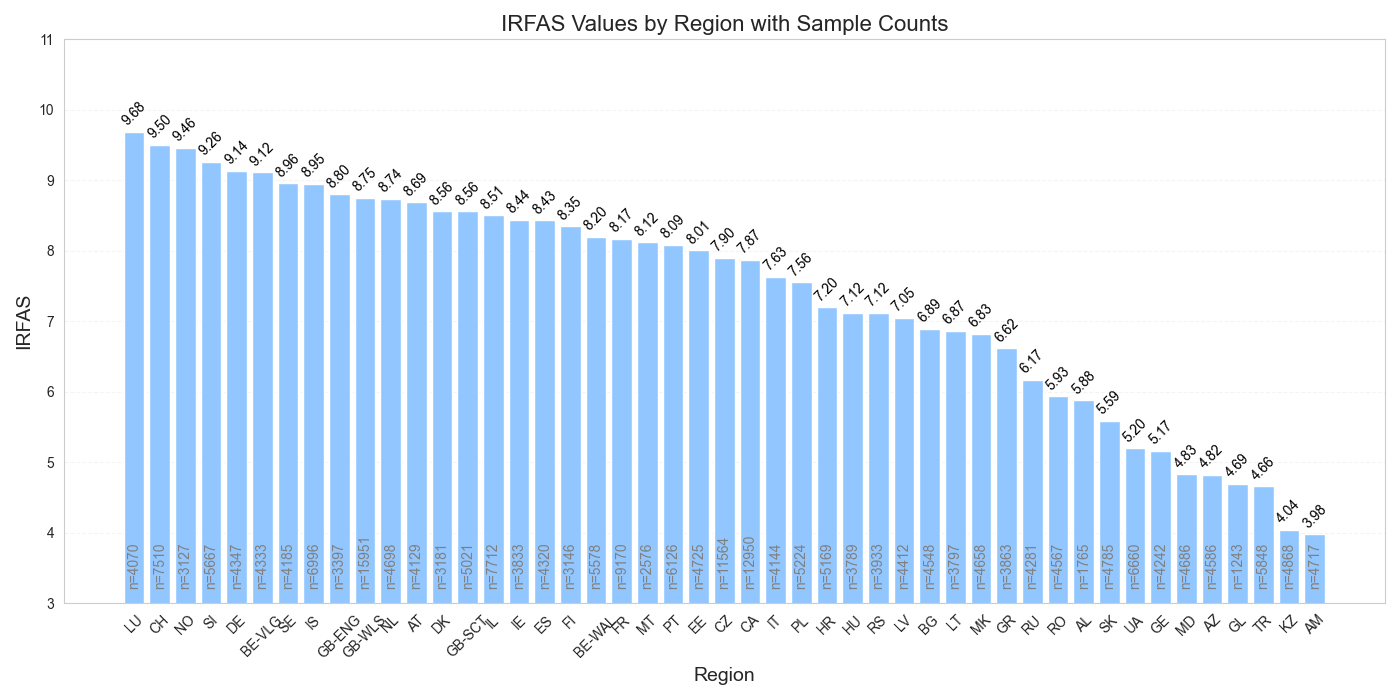
\includegraphics[width=0.8\textwidth]{IRFAS_histogram.png}
    \caption{Average IRFAS score by region. The black number indicates the IRFAS score, while the grey number (n=) represents the sample size for each region.}
    \label{fig:IRFAS_histogram}
\end{figure}

% \begin{table}[h]
% \centering
% \begin{tabular}{|l|l@{}|}
% \toprule
% \textbf{Variable Name} & \textbf{Description} \\
% \midrule
% \texttt{fasfamcar}   & Does your family own a car, van or truck? \\
% \texttt{fasbedroom}  & Do you have your own bedroom for yourself? \\
% \texttt{fascompu}    & Number of computers (PCs, laptops, tablets) in the household \\
% \texttt{fasbathr}    & Number of bathrooms in the home (with bath or shower) \\
% \texttt{fasdishw}    & Does your family have a dishwasher? \\
% \texttt{fasholid}    & How many times did your family travel abroad for holidays last year? \\
% \bottomrule
% \end{tabular}
% \caption{Variable descriptions for Family Affluence Scale (FAS) items}
% \label{tab:FAS_variables}
% \end{table}


As part of this report, we have decided to focus on data from Ukraine, denoted as region UA in the dataset, or country number 804000. Data acquisition in Ukraine was performed in April and May 2018 using pen-and-paper surveys. Since we are focusing on only one country, it makes sense to ignore columns that have a single value throughout, such as \texttt{HBSC, cluster, countryno, adm, month,} and \texttt{year}. Alongside these, we will exclude any metadata like IDs or data weights from the causal analysis.

Moreover, most of the variables are categorical or discrete. All continuous variables have categorical counterparts, so we will use those instead. Generally speaking, demographics [Table \ref{tab:hbsc_variables_grouped}] and the rest of the variables can be important and serve as confounders or mediators. Therefore, we decided to examine each category closely and select variables that contribute most to analyzing the reasons and causes of bullying in children. We keep in mind that we are interested in variables that influence bullying.

Table \ref{tab:hbsc_variables_grouped} reflects a larger subset of variables considered for the analysis. However, we also focus on a subset of 27 variables: \texttt{bulliedothers, beenbullied, cbulliedothers, cbeenbullied, fight12m, lifesat, famhelp, famsup, famtalk, famdec, friendhelp, friendcounton, friendshare, friendtalk, likeschool, schoolpressure, studtogether, studhelpful, studaccept, teacheraccept, teachercare, teachertrust, timeexe, talkfather, talkstepfa, talkmother,} and \texttt{talkstepmo}. We deem these variables to provide the most information on the subject of bullying and cyberbullying.

We exclude deterministic variables such as \texttt{IRFAS, IRRELFAS\_LMH, MBMI, IOTF4,} and \texttt{oweight\_who} from our analysis, alongside variables irrelevant to bullying, such as those related to sexual health and health behaviours like smoking, drinking, and food consumption (see Table \ref{tab:hbsc_variables_grouped}).


% \begin{longtable}{lllllllllllllllll}
\caption{Summary table of variables from the HBSC dataset, where each variable is assigned to a category depending on the data it represents} \label{tab:hbsc_variables_groups} \\
\toprule
Category & Demographics & Metadata & Family Affluence Scale & Health & Well-being & Somatic Symptoms & Health Behaviors & Body Measures & School Experience & Violence and Bullying & Peer Support & Emotional Communication Preferences & Sexual Health & Migration Background & Household Composition & Parental Employment & Parent�Child Communication & Family Support \\
\midrule
\endfirsthead
\caption[]{Summary table of variables from the HBSC dataset, where each variable is assigned to a category depending on the data it represents} \\
\toprule
Category & Demographics & Metadata & Family Affluence Scale & Health & Well-being & Somatic Symptoms & Health Behaviors & Body Measures & School Experience & Violence and Bullying & Peer Support & Emotional Communication Preferences & Sexual Health & Migration Background & Household Composition & Parental Employment & Parent�Child Communication & Family Support \\
\midrule
\endhead
\midrule
\multicolumn{17}{r}{Continued on next page} \\
\midrule
\endfoot
\bottomrule
\endlastfoot
Variables & HBSC, seqno_int, cluster, countryno, region, id1, id2, id3, id4, weight, adm, month, year, age, agecat, sex, grade, monthbirth, yearbirth & fasfamcar, fasbedroom, fascomputers, fasbathroom, fasdishwash, fasholidays, IRFAS, IRRELFAS_LMH & health, lifesat, MBMI, IOTF4, oweight_who & headache, stomachache, backache, feellow, irritable, nervous, sleepdificulty, dizzy, thinkbody & physact60, timeexe, breakfastwd, breakfastwe, fruits_2, vegetables_2, sweets_2, softdrinks_2, fmeal, toothbr, smokltm, smok30d_2, alcltm, alc30d_2, drunkltm, drunk30d, cannabisltm_2, cannabis30d_2 & bodyweight, bodyheight & likeschool, schoolpressure, studtogether, studhelpful, studaccept, teacheraccept, teachercare, teachertrust & bulliedothers, beenbullied, cbulliedothers, cbeenbullied, fight12m, injured12m & friendhelp, friendcounton, friendshare, friendtalk & emconlfreq1, emconlfreq2, emconlfreq3, emconlfreq4, emconlpref1, emconlpref2, emconlpref3, emcsocmed1, emcsocmed2, emcsocmed3, emcsocmed4, emcsocmed5, emcsocmed6, emcsocmed7, emcsocmed8, emcsocmed9 & hadsex, agesex, contraceptcondom, contraceptpill & countryborn, countrybornmo, countrybornfa & motherhome1, fatherhome1, stepmohome1, stepfahome1, fosterhome1, elsehome1_2 & employfa, employmo, employnotfa, employnotmo & talkfather, talkstepfa, talkmother, talkstepmo & famhelp, famsup, famtalk, famdec \\
\end{longtable}


% \begin{longtable}{lrrrrrrr}
\caption{Crosstabulation of responses to how easy it is for respondents to talk to their father and stepfather about things that really bother them. Values represent the number of respondents selecting each pair of response categories. Responses range from 1 (Very easy) to 4 (Very difficult), reflecting increasing difficulty. The values 0 and 5 represent non-substantive responses: 0 indicates a missing response, and 5 corresponds to "Dont have or see" the person in question.} \label{tab:father_stepfather_support_pivot} \\
\toprule
talkstepfa & 0 & 1 & 2 & 3 & 4 & 5 & Total \\
talkfather &  &  &  &  &  &  &  \\
\midrule
\endfirsthead
\caption[]{Crosstabulation of responses to how easy it is for respondents to talk to their father and stepfather about things that really bother them. Values represent the number of respondents selecting each pair of response categories. Responses range from 1 (Very easy) to 4 (Very difficult), reflecting increasing difficulty. The values 0 and 5 represent non-substantive responses: 0 indicates a missing response, and 5 corresponds to "Dont have or see" the person in question.} \\
\toprule
talkstepfa & 0 & 1 & 2 & 3 & 4 & 5 & Total \\
talkfather &  &  &  &  &  &  &  \\
\midrule
\endhead
\midrule
\multicolumn{8}{r}{Continued on next page} \\
\midrule
\endfoot
\bottomrule
\endlastfoot
0 & 2712 & 267 & 389 & 252 & 146 & 1487 & 5253 \\
1 & 20628 & 4954 & 2997 & 2028 & 1247 & 41923 & 73777 \\
2 & 18105 & 944 & 4816 & 3012 & 1582 & 49887 & 78346 \\
3 & 7975 & 503 & 1438 & 3269 & 1627 & 25477 & 40289 \\
4 & 3322 & 302 & 599 & 679 & 2714 & 11394 & 19010 \\
5 & 2045 & 921 & 1661 & 1087 & 1311 & 8159 & 15184 \\
Total & 54787 & 7891 & 11900 & 10327 & 8627 & 138327 & 231859 \\
\end{longtable}




% \begin{longtable}{rrrrrrr}
\caption{Crosstabulation of responses to how easy it is for respondents to talk to their mother and stepmother about things that really bother them. Values represent the number of respondents selecting each pair of response categories. Responses range from 1 (Very easy) to 4 (Very difficult), reflecting increasing difficulty. The values 0 and 5 represent non-substantive responses: 0 indicates a missing response, and 5 corresponds to "Dont have or see" the person in question.} \label{tab:mother_stepmother_support_pivot} \\
\toprule
0 & 1 & 2 & 3 & 4 & 5 & Total \\
\midrule
\endfirsthead
\caption[]{Crosstabulation of responses to how easy it is for respondents to talk to their mother and stepmother about things that really bother them. Values represent the number of respondents selecting each pair of response categories. Responses range from 1 (Very easy) to 4 (Very difficult), reflecting increasing difficulty. The values 0 and 5 represent non-substantive responses: 0 indicates a missing response, and 5 corresponds to "Dont have or see" the person in question.} \\
\toprule
0 & 1 & 2 & 3 & 4 & 5 & Total \\
\midrule
\endhead
\midrule
\multicolumn{7}{r}{Continued on next page} \\
\midrule
\endfoot
\bottomrule
\endlastfoot
1749 & 188 & 226 & 149 & 69 & 902 & 3283 \\
30505 & 5116 & 3667 & 3092 & 2487 & 71032 & 115899 \\
17244 & 671 & 3755 & 2570 & 1926 & 48747 & 74913 \\
4830 & 340 & 608 & 1913 & 1107 & 15244 & 24042 \\
1728 & 181 & 250 & 217 & 1622 & 5278 & 9276 \\
712 & 368 & 358 & 200 & 203 & 2605 & 4446 \\
56768 & 6864 & 8864 & 8141 & 7414 & 143808 & 231859 \\
\end{longtable}

\subsection{Data Issues and Preprocessing}
\begin{itemize}
  \item   Missing data is handled for us so that we won't get stuck on it for too long. In the original report \cite{HBSC2018OA_ed1}, randomly missing values coded as sysmiss and represented as 'Nones' in the dataset are shown. Besides that, there are also more types of missingness observed in data, such as "Missing due to skip pattern"(99) or "Missing due to inconsistent answer"(-99). Fortunately, 99 and -99 missingness types are not present in our subset of data. Since the rest is missing completely at random, by assumption, we drop the records with missing values, accounting for the qualities of FCI to handle selection bias\cite{ZHANG20081873} that might occur after such data manipulation. 
  \item For the few continuous ones, we selected their discrete counterparts where available. All categorical string variables were label-encoded into integers. 
  \item  The resulting sample size for Ukraine is 6,660 records. This is sufficient to produce statistically meaningful results, even after removing records with missing values. 
  \item We acknowledge that using only Ukrainian data limits generalizability.
\end{itemize}


% \subsection{Scientific Question}
% Relationship of social integration of a child and aggression levels channeled through bullying and participation in fights.

% \begin{figure}[h]
%   \centering
%   \begin{subfigure}[t]{0.48\textwidth}
%     \centering
%     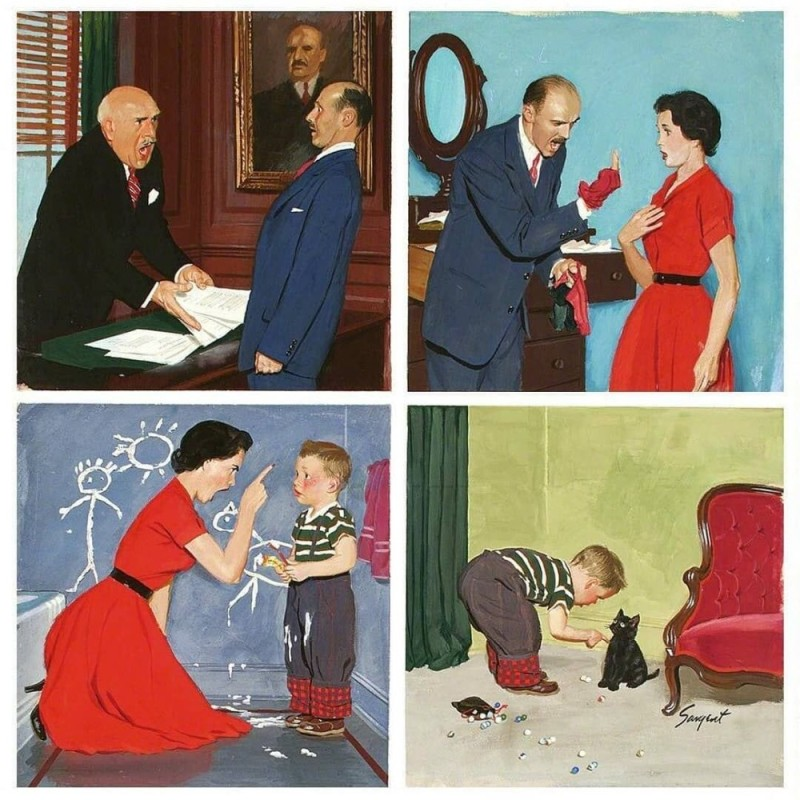
\includegraphics[width=\textwidth]{Report/pics/cycle of abuse.png}
%     \caption{Inspirational diagram for forming a scientific question.}
%   \end{subfigure}
%   \hfill
%   \begin{subfigure}[t]{0.48\textwidth}
%     \centering
%     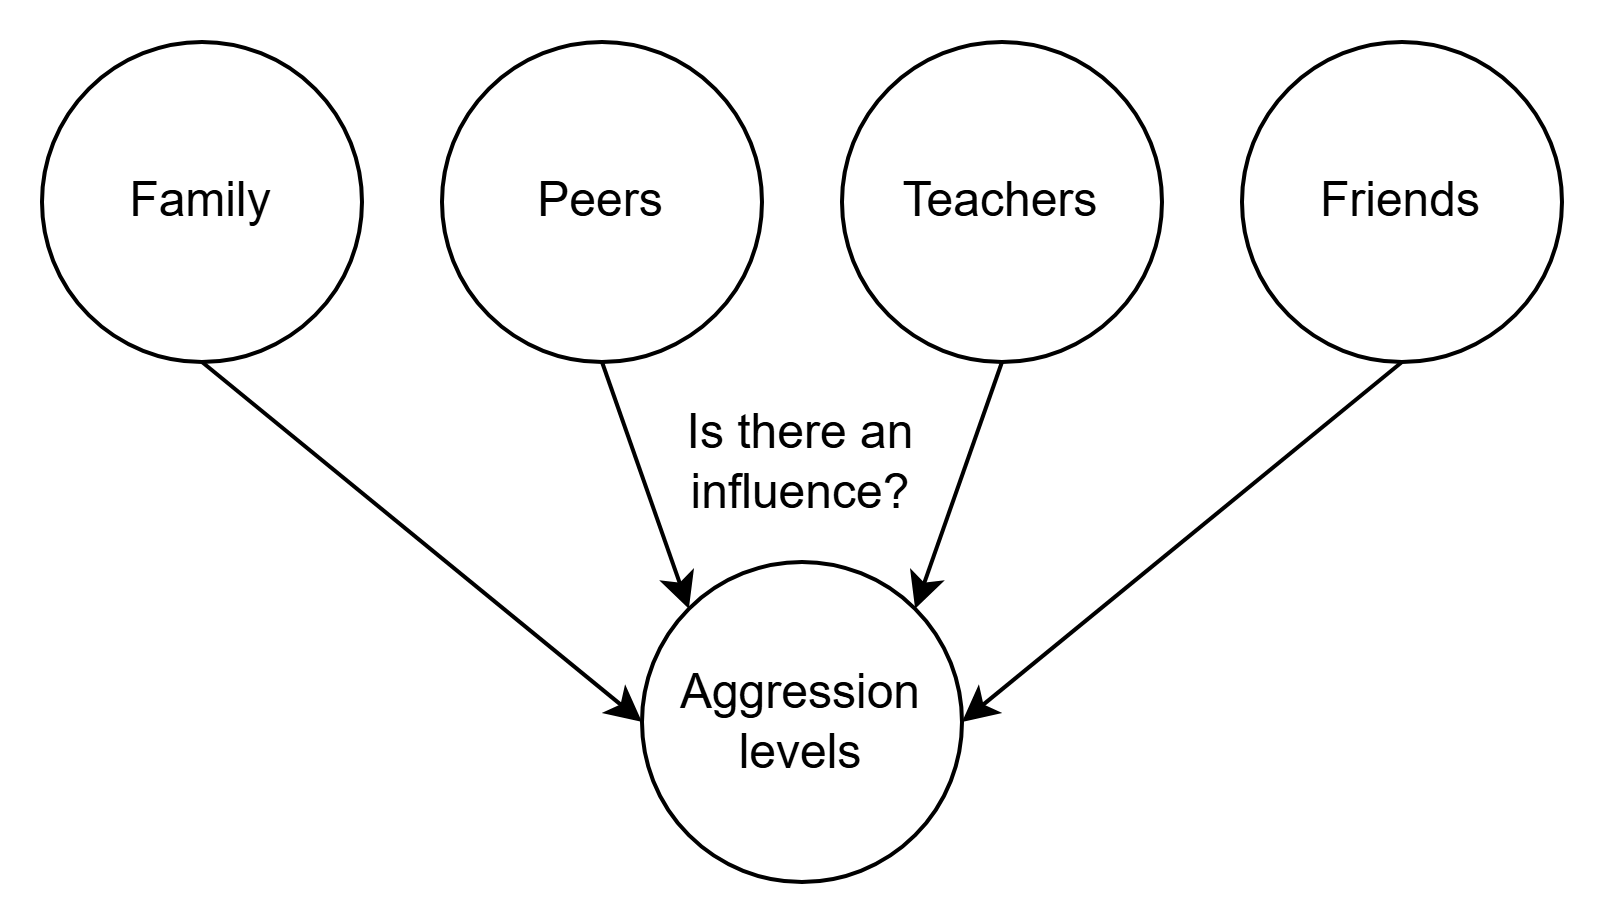
\includegraphics[width=\textwidth]{Report/pics/scheme for scientific question.png}
%     \caption{Conceptual scheme illustrating the scientific question.}
%   \end{subfigure}
%   \caption{The first figure serves as inspiration, while the second is a vague schematic formulation of our scientific question.}
% \end{figure}
\end{document}